
\documentclass{article}

\usepackage{graphicx}
\usepackage{titlesec}
\usepackage{float}
\usepackage{listings}
\usepackage{color}

\setcounter{secnumdepth}{4}


\definecolor{dkgreen}{rgb}{0,0.6,0}
\definecolor{gray}{rgb}{0.5,0.5,0.5}
\definecolor{mauve}{rgb}{0.58,0,0.82}

\lstset{frame=tb,
  language=C,
  aboveskip=3mm,
  belowskip=3mm,
  showstringspaces=false,
  columns=flexible,
  basicstyle={\small\ttfamily},
  numbers=none,
  numberstyle=\tiny\color{gray},
  keywordstyle=\color{blue},
  commentstyle=\color{dkgreen},
  stringstyle=\color{mauve},
  breaklines=true,
  breakatwhitespace=true,
  tabsize=3
}

\titleformat{\paragraph}
{\normalfont\normalsize\bfseries}{\theparagraph}{1em}{}
\titlespacing*{\paragraph}
{0pt}{3.25ex plus 1ex minus .2ex}{1.5ex plus .2ex}

\parskip=12pt

\begin{document}

\title{Lab 1: Design of Robotic Systems}
\date{January 26, 2017}
\author{Wu, Yichen \\504294181\\  \\Collaborator: \\Yaofang Zhang \\004446568\\ \\EE183D}

\maketitle

\section{Introduction}

In this lab, we modeled the mechanical linkage of a human leg (Fig. 1), with 3 degrees of freedom at hip and 1 degree of freedom at knee. 

\begin{figure}[H]
\centering
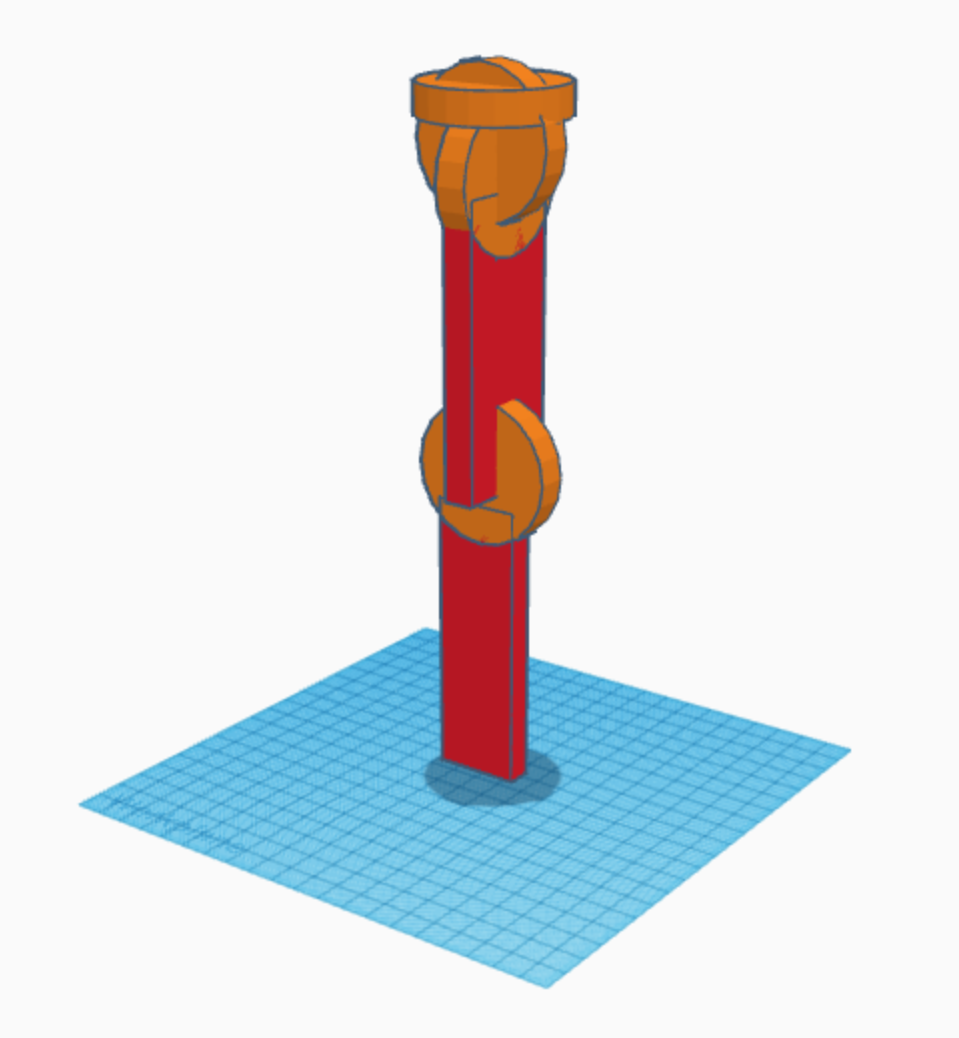
\includegraphics[width=250pt]{leg}
\end{figure}

Low birth weight rate in non-smoker group is $4.1\%$, compared to $7.8\%$ in smoker group. This supports the association between low birth rate and mom's smoking habbit.  

\section{Summary}

This lab covered the concept and attributes of categorical and numerical data.  

\end{document}

